% !TeX spellcheck = en_US

\chapter{Trees}

\section {General Trees}

A \textbf{tree} is an abstract data type that organize that elements hierarchically.

A tree is \textbf{ordered} if there is a meaningful order among the children of each node.

\section{Binary Tree}

A \textbf{binary tree} is an ordered tree with the following properties :
....... to finish

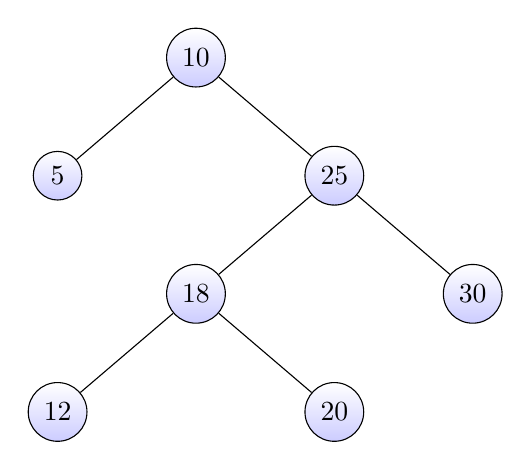
\begin{tikzpicture}[sibling distance=10em,
every node/.style = {shape=circle,
	draw, align=center,
	top color=white, bottom color=blue!20}]]
\node {10}
child { node {5} }
child { node {25}
	child { node {18}
		child { node {12} }
		child { node {20} } }
	child { node {30} } };
\end{tikzpicture}

\section{Tries (Prefix trees)}

A \textbf{trie} is a variant of a n-ary tree in which characters are stored at each node.  


